% Lab 1: Analog Simulation
% !TEX program = lualatex
% LaTeX template for ECE 486 Lab

\documentclass[a4paper]{article}
\usepackage{indentfirst}
\usepackage{fancyhdr}
\usepackage{enumerate}
\usepackage{fontenc}
\usepackage{graphicx}
\usepackage{caption}
\usepackage{mathtools} % load AMS maths
\usepackage{amsmath}  % for math spacing
\usepackage{amssymb}  % for math spacing
\usepackage{fontspec}
\usepackage{lastpage}
\usepackage[margin=1in]{geometry} % an easy way to change page layout
                                  % Thanks to Brady Salz 
\setlength{\parskip}{1em} % 设置段落间距
% ----------------------------
%            Tikz
% ----------------------------

\usepackage{tikz}
\usetikzlibrary{shapes,arrows}
\usepackage{verbatim}

% ----------------------------

% \usepackage{kpfonts-otf}
% \usepackage{libertinus-otf}
% \usepackage{plex-otf}
\newcommand{\D}{\text{d}}

\usepackage{mathptmx}
\setmainfont{Times New Roman}

\newcommand{\score}{\hfill \underline{\hspace{0.65cm}}\,/} % for score underline
\newcommand\RR{\textsuperscript{\textregistered}~} % for registered mark
\newcommand{\EXERCISE}[1]{\subsection*{Ex \textit{#1}.}}
\newcommand{\EXERCISENAME}[2]{\subsection*{Ex #1: \textit{#2}}}
\newcommand\makeMyTitle{\maketitle \thispagestyle{firstPage}}

\pagestyle{fancy}
\fancyhf{}
\fancyhead[C]{}
\fancyhead[L]{\it Lab \LABNUMBER: \LABTITLE}
\fancyhead[R]{\it \today}
\fancyfoot[L]{\textit{Tiantian Zhong}}
\fancyfoot[C]{\thepage/\pageref{LastPage}}
\fancyfoot[R]{\textit{0000000000}}
\renewcommand{\headrulewidth}{0.5pt}
\renewcommand{\footrulewidth}{0.5pt}

\fancypagestyle{firstPage}{
    \fancyhf{}
    \fancyhead[L]{\it ECE 486 \\\it Control Systems}
    \fancyhead[C]{}
    \fancyhead[R]{\it Fall 2022 \\\it  ZJU-UIUC Institute}
    \fancyfoot[L]{}
    \fancyfoot[C]{\thepage/\pageref{LastPage}}
    \fancyfoot[R]{}
    \renewcommand{\headrulewidth}{0.5pt}
    \renewcommand{\footrulewidth}{0.5pt}
}

\newcommand{\E}{\text{e}}
% \newcommand{\Diff}{\text{d}}
\renewcommand{\Re}{\text{Re}}
\renewcommand{\Im}{\text{Im}}

\title{\textbf{Lab Report} \\ Lab \#\LABNUMBER: \textsc{\LABTITLE}}
\author{\AUTHOR \\ \ID}
\date{\today}

\def\AUTHOR{Tiantian Zhong}
\def\ID{3200110643}
% \def\REPORTTITLE{\textsc{\LABTITLE}}

\everymath{\displaystyle}

% ----------------------------
%      Tikz Configuration
% ----------------------------

\tikzstyle{block} = [draw, rectangle, 
minimum height=3em, minimum width=3em]
\tikzstyle{sum} = [draw, circle, node distance=1cm]
\tikzstyle{input} = [coordinate]
\tikzstyle{output} = [coordinate]
\tikzstyle{pinstyle} = [pin edge={to-,thin,black}]
\tikzstyle{triangle} = [isosceles triangle, draw, minimum height = 3em]
\newcommand\K{\text{k}} % kilo = 1000
\date{    \begin{tabular}{rl}
    Experiment Date: &  \EXPDATE \\
    Report Date: & \RPTDATE
\end{tabular} }


\def\LABNUMBER{1}
\def\LABTITLE{Analog Simulation}
\newcommand\K{\text{k}}

\begin{document}

\makeMyTitle

\section{Prelab Exercises}
\EXERCISE{a}

From Newton's 3rd law, I derive the following equation:
\begin{align*}
  f &= ma_{tot} + bv + kx \\
  a_{tot} &= \frac{\D^2}{\D t^2} x \\
  v &= \frac{\D}{\D t} x
\end{align*}
thus the ODE should look like this:
\begin{equation*}
  f(t)=m\ddot{x}(t)+b\dot{x}(t)+kx(t)
\end{equation*}

Substituting the values for $m$, $b$, $k$, and $f$ I obtain
\begin{equation}\label{eq-ode}
  f(t)=2\ddot{x}(t)+0.7\dot{x}(t)+x(t).
\end{equation}

% End of Ex a.

\EXERCISE{b}

Laplace Transform of 2nd-order ODE (with zero initial condition) in Equation
\refeq{eq-ode}:
\begin{align*}
  f(t)=2\ddot{x}(t)+0.7\dot{x}(t)+x(t) \leftrightarrow F(s)=2 s^2 X(s)+
                                                            0.7 sX(s) + X(s)
\end{align*}
and move $s^2 X$ to LHS and $F$ to RHS:
\begin{equation} 
  s^2 X = \frac{0.7}{2}sX+\frac{1}{2}X-\frac{1}{2}F
  \label{eq-diagram}
\end{equation}
which gives the diagram in Figure \ref{pic-diagram}.
\begin{figure}[h!]
  \centering
  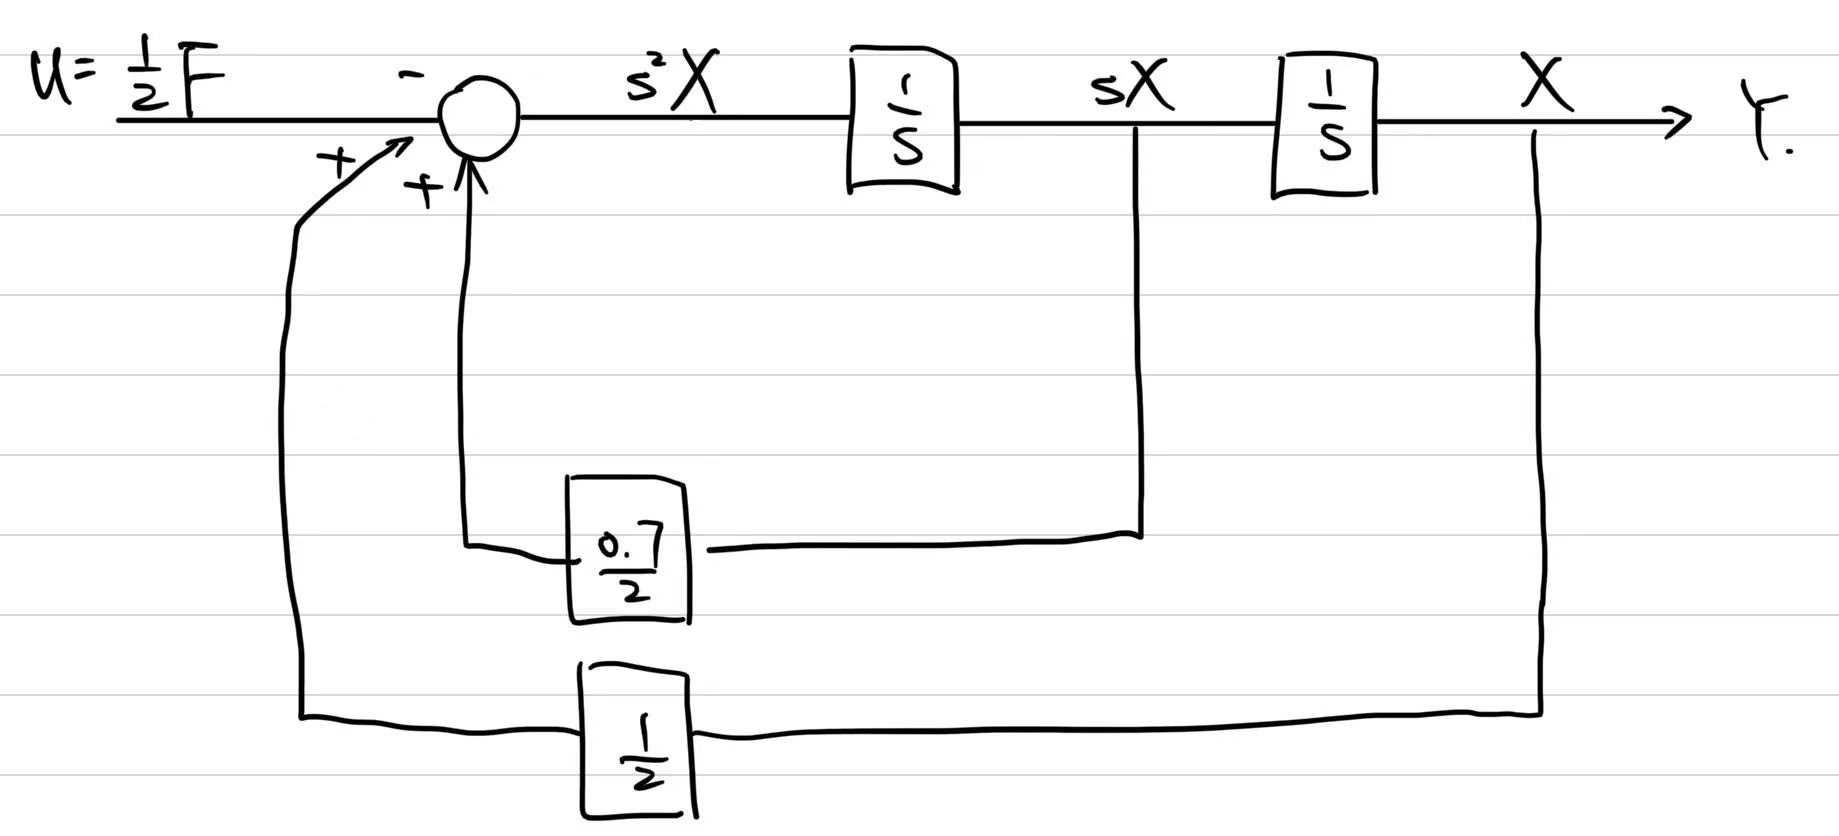
\includegraphics[width=0.7\textwidth]{pics/prelab-blkdgm.jpg}
  \caption{Block diagram for Equation \refeq{eq-diagram}}
  \label{pic-diagram}
\end{figure}
% % !TEX program = lualatex
% LaTeX template for ECE 486 Lab

\documentclass[a4paper]{article}
\usepackage{indentfirst}
\usepackage{fancyhdr}
\usepackage{enumerate}
\usepackage{fontenc}
\usepackage{graphicx}
\usepackage{caption}
\usepackage{mathtools} % load AMS maths
\usepackage{amsmath}  % for math spacing
\usepackage{amssymb}  % for math spacing
\usepackage{fontspec}
\usepackage{lastpage}
\usepackage[margin=1in]{geometry} % an easy way to change page layout
                                  % Thanks to Brady Salz 
\setlength{\parskip}{1em} % 设置段落间距
% ----------------------------
%            Tikz
% ----------------------------

\usepackage{tikz}
\usetikzlibrary{shapes,arrows}
\usepackage{verbatim}

% ----------------------------

% \usepackage{kpfonts-otf}
% \usepackage{libertinus-otf}
% \usepackage{plex-otf}
\newcommand{\D}{\text{d}}

\usepackage{mathptmx}
\setmainfont{Times New Roman}

\newcommand{\score}{\hfill \underline{\hspace{0.65cm}}\,/} % for score underline
\newcommand\RR{\textsuperscript{\textregistered}~} % for registered mark
\newcommand{\EXERCISE}[1]{\subsection*{Ex \textit{#1}.}}
\newcommand{\EXERCISENAME}[2]{\subsection*{Ex #1: \textit{#2}}}
\newcommand\makeMyTitle{\maketitle \thispagestyle{firstPage}}

\pagestyle{fancy}
\fancyhf{}
\fancyhead[C]{}
\fancyhead[L]{\it Lab \LABNUMBER: \LABTITLE}
\fancyhead[R]{\it \today}
\fancyfoot[L]{\textit{Tiantian Zhong}}
\fancyfoot[C]{\thepage/\pageref{LastPage}}
\fancyfoot[R]{\textit{0000000000}}
\renewcommand{\headrulewidth}{0.5pt}
\renewcommand{\footrulewidth}{0.5pt}

\fancypagestyle{firstPage}{
    \fancyhf{}
    \fancyhead[L]{\it ECE 486 \\\it Control Systems}
    \fancyhead[C]{}
    \fancyhead[R]{\it Fall 2022 \\\it  ZJU-UIUC Institute}
    \fancyfoot[L]{}
    \fancyfoot[C]{\thepage/\pageref{LastPage}}
    \fancyfoot[R]{}
    \renewcommand{\headrulewidth}{0.5pt}
    \renewcommand{\footrulewidth}{0.5pt}
}

\newcommand{\E}{\text{e}}
% \newcommand{\Diff}{\text{d}}
\renewcommand{\Re}{\text{Re}}
\renewcommand{\Im}{\text{Im}}

\title{\textbf{Lab Report} \\ Lab \#\LABNUMBER: \textsc{\LABTITLE}}
\author{\AUTHOR \\ \ID}
\date{\today}

\def\AUTHOR{Tiantian Zhong}
\def\ID{3200110643}
% \def\REPORTTITLE{\textsc{\LABTITLE}}

\everymath{\displaystyle}

% ----------------------------
%      Tikz Configuration
% ----------------------------

\tikzstyle{block} = [draw, rectangle, 
minimum height=3em, minimum width=3em]
\tikzstyle{sum} = [draw, circle, node distance=1cm]
\tikzstyle{input} = [coordinate]
\tikzstyle{output} = [coordinate]
\tikzstyle{pinstyle} = [pin edge={to-,thin,black}]
\tikzstyle{triangle} = [isosceles triangle, draw, minimum height = 3em]
\newcommand\K{\text{k}} % kilo = 1000
\date{    \begin{tabular}{rl}
    Experiment Date: &  \EXPDATE \\
    Report Date: & \RPTDATE
\end{tabular} }

\begin{document}
\def\LABNUMBER{1}
\def\LABTITLE{Analog Simulation}
\begin{tikzpicture}[auto, node distance=2cm]

    % We start by placing the blocks
    % \node [input, name=input] {};
    % \node [sum, right of=input] (sum) {};
    % \node [triangle, right of=sum] (controller) {$G_c(s)$};
    % \node [block, right of=controller,
    %         node distance=3cm] (system) {$G_p(s)$};
    % % We draw an edge between the controller and system block to 
    % % calculate the coordinate u. We need it to place the measurement block. 
    % \draw [->] (controller) -- node[name=u] {$U$} (system);
    % \node [sum, right of=system, node distance=2cm] (disturbance) {};
    % \node [block, above of=disturbance] (g_d) {$G_d(s)$};
    % \node [input, left of=g_d] (dist_input){$D$};
    % \node [output, right of=disturbance] (output) {};
    % \node [block, below of=u] (measurements) {$G_m(s)$};

    % % Once the nodes are placed, connecting them is easy. 
    % \draw [draw,->] (input) -- node {$Y_{sp}$} (sum);
    % \draw [->] (sum) -- node {$E$} (controller);
    % \draw [->] (system) -- node {$Y_u$} (disturbance);
    % \draw [->] (disturbance) -- node [name=y] {$Y$}(output);
    % \draw [->] (g_d) -- node {$Y_d$} (disturbance);
    % \draw [draw, ->] (dist_input) -- node {$D$} (g_d);
    % \draw [->] (y) |- (measurements);
    % \draw [->] (measurements) -| node[pos=0.99] {$-$} 
    %     node [near end] {$Y_m$} (sum);

    \node [input, name=input] {};
    \node [sum, right of=input] (sum) {};
    \draw [->] (input) -- node[name=input]{$U(s)$} (sum) node [left of = sum, above of = sum] {$+$};
    \node [block, name=diff1, right of=sum] (diff1) {$\frac{1}{s}$};
    \draw [->] (sum) -- node[name=s2x] {$s^2 X$} (diff1);
    \node[block, below of = diff1] (amp1){$a_0$};
    \node[block, below of = amp1] (amp2){$a_1$};

    \node [block, name=diff2, right of=diff1] (diff2) {$\frac{1}{s}$};
    \draw [->] (diff1) -- node[name=sx] {$sX$} (diff2);

    \node [output, right of = diff2](output) {};
    \draw [->] (diff2) -- node[name=x] {$X$} (output);

    \draw [-] (sx) |- (amp1);
    \draw [->] (amp1) -| node[pos=0.99] {$-$} 
         node [near end, name=measurement1] {$Y_m$} (sum);

    \draw [-] (x) |- (amp2);
    \draw [->] (amp2) -| node[left of = measurement1] {$-$}
         node [near end] {$Y_m$} (sum);
\end{tikzpicture}

     
\end{document}

% End of Ex b.
\pagebreak
\EXERCISE{c}

For Figure 2(b) in the manual I can derive a group of equations based on KVL,
\begin{align}
   q_C &= Ce_o(t) \\
  e_i(t) - e_o(t) &= i(t)R \\
  \D q_C &= i(t)\D t
\end{align}
which gives
\begin{align*}
  &e_i(t) - \frac{q_C}{C} = i(t) R \\
\Rightarrow   &e_i(t) - \frac{1}{C}\int i(t)\D t- i(t)R = 0.
\end{align*}

%End of Ex c.

\pagebreak\section{Lab Exercises}
\EXERCISENAME{1}{Solving Differential Equations using Analog Computer}

\subsubsection*{Damp Coefficient $b=0.7$}

Prelab exercise provides a 2nd-order ODE
\[ m\ddot{x} + b\dot{x} + kx = F \]
which, using Laplace Transform, can be represented as 
\[ s^2 X(s) + \frac{b}{m}sX(s) + \frac{k}{m}X(s) = \frac{F}{m}. \]

For step 2, I found the I/O relationship at \texttt{adder1} can be represented
as 
\[ Y = -\frac{R_f}{F_1}x_1 - \frac{R_f}{F_2}x_2\]
and substituting $x_1, x_2$ with its corresponding signals $-\dot{x}, F(t)=0.5$
I obtain
\[ \frac{F(t)-b\dot{x}}{m}=\frac{0.5-0.7\dot{x}}{2}=-\dot{x}\frac{10\K}{28.6\K}
+0.5\frac{10\K}{20\K} \]
which matches the original parameter in the SIMUNLINK model.

This step produces a plot of $x(t)$ and $x'(t)$ over time, which is shown in
Figure \ref{pic-b0.7} and \ref{pic-b0.7_2}.

\begin{figure}[h!]
  \begin{minipage}{0.45\linewidth}
    \centering
    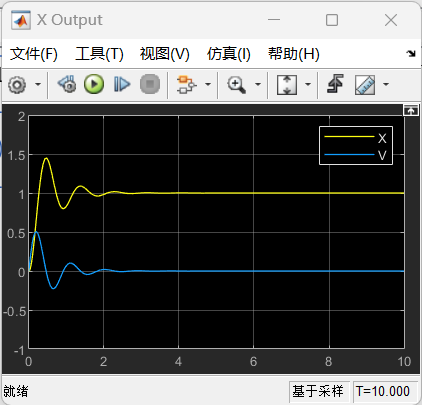
\includegraphics[width=0.8\textwidth]{pics/ex1-b0.7.png}
    \caption{Function $x(t)$ and $v(t)$ with the change of $t$; generated by 
            SIMULINK model}
    \label{pic-b0.7}
  \end{minipage}
  \begin{minipage}{0.45\linewidth}
    \centering
    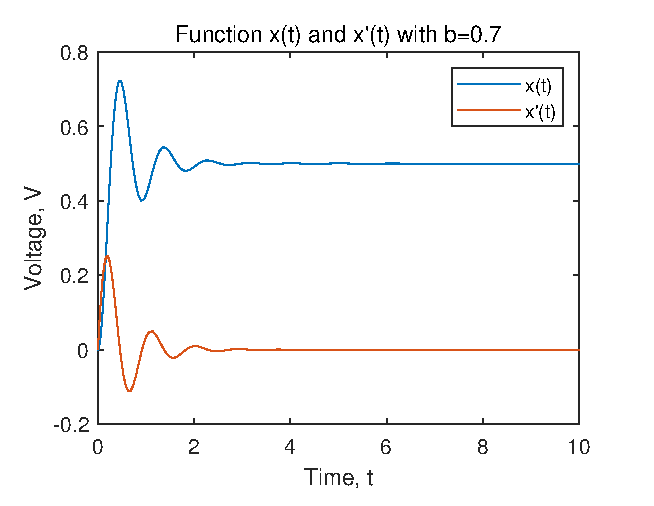
\includegraphics[scale=0.7]{pics/ex1-b0.7-plot.eps}
    \caption{Function $x(t)$ and $v(t)$ with the change of $t$; plotted by 
            MATLAB}
    \label{pic-b0.7_2}
    
  \end{minipage}
  
\end{figure}

\subsubsection*{Damp Coefficient $b=1$}

Let's focus on $R_1$ in Figure \ref{pic-r1}.

\begin{figure}[h!]
  \centering
  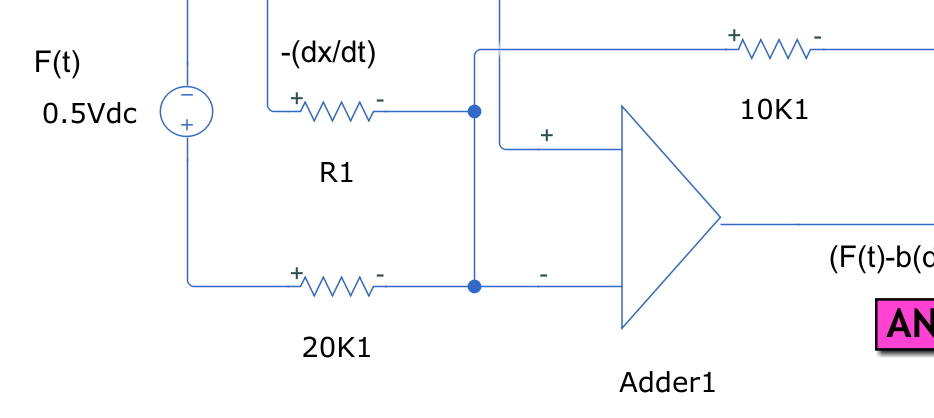
\includegraphics[scale=0.5]{pics/adder1-r1.png}
  \caption{Block diagram near \texttt{adder1}}
  \label{pic-r1}
\end{figure}

As is discussed above, the I/O relationship of \texttt{adder1} is
\[ \frac{F(t)-b\dot{x}}{m}=\frac{0.5-\dot{x}}{2}=-\dot{x}\frac{10\K}{R_1}
+0.5\frac{10\K}{20\K} \]
which yields
\[\frac{1}{2}=\frac{10\K}{R_1}.\]

Thus here I take $R_1=20\K\Omega$. The plots for function $x_{b=1}(t)$
and $x'_{b=1}(t)$ is shown in Figure \ref{pic-b1} and \ref{pic-b1-plot}.

\begin{figure}[htbp]
  \begin{minipage}{0.49\linewidth}
    \centering
    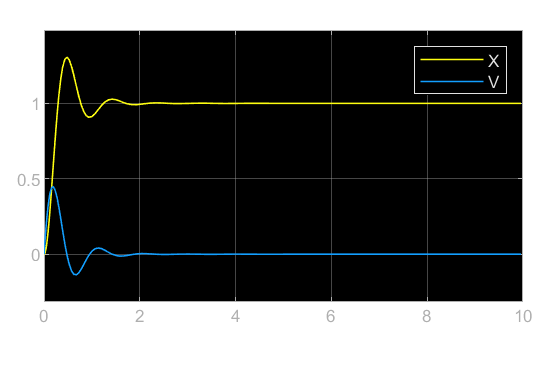
\includegraphics[width=0.99\textwidth]{pics/ex1-b1.eps}
    \caption{Function $x_{b=1}(t)$ and $x'_{b=1}(t)$ with the change of $t$;
    generated by SIMULINK model}
    \label{pic-b1}
  \end{minipage}
  \begin{minipage}{0.49\linewidth}
    \centering
    \includegraphics[width=0.99\textwidth]{pics/ex1-b1-plot.eps}
    \caption{Function $x(t)$ and $v(t)$ with the change of $t$; plotted by 
    MATLAB}
    \label{pic-b1-plot}
  \end{minipage}
  
\end{figure}

\subsubsection*{Discussion about the Changes in Response}

\textbf{For the changes with $b$}, I derived an expression for $R_1$ in Figure
\ref{pic-r1}:
\[R_1=10\K \frac{m}{b}\]
which indicates that I can explore the change of functions with different
$R_1$. It is concluded that with an increasing $R_1$, i.e. decreasing $b$,
\begin{enumerate}
  \item the system will reach its steady state with longer time.
  \item there will be a higher maximum value of system response.
  \item frequency remains unchanged.
\end{enumerate}

I plotted function $x(t)$ for different $R_1$, which is shown in
Figure \ref{pic-m-b}.

\begin{figure}[htbp]
  \centering
  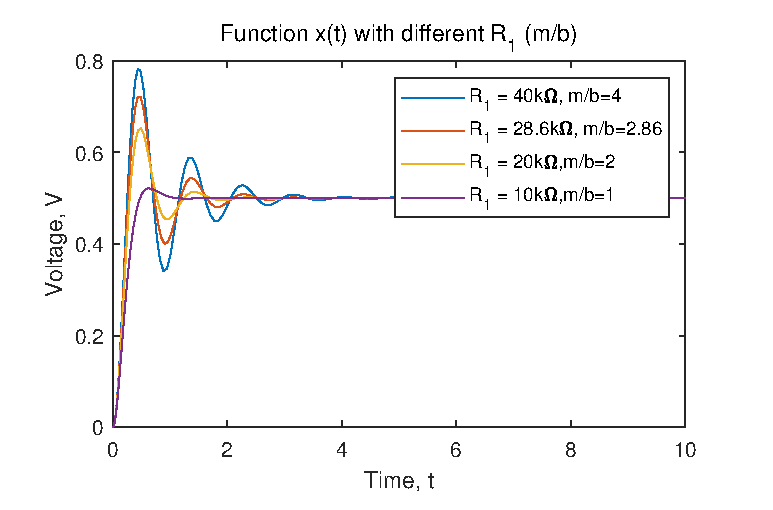
\includegraphics[width=0.7\textwidth]{pics/change-m-b.eps}
  \caption{Function $x(t)$ with different values of $\frac{m}{b}$}
  \label{pic-m-b}
\end{figure}

\textbf{For the changes with $F(t)$}, the steady state response is exactly the
value of $F(t)$. As $F(t)$ changes, the response changes accordingly.

\textbf{For the changes with $k$}, similar as before I derived an expression
for $R_2$, which is 
\[R_2=10\K \frac{m}{k}.\]

\begin{figure}[htbp]
  \centering
  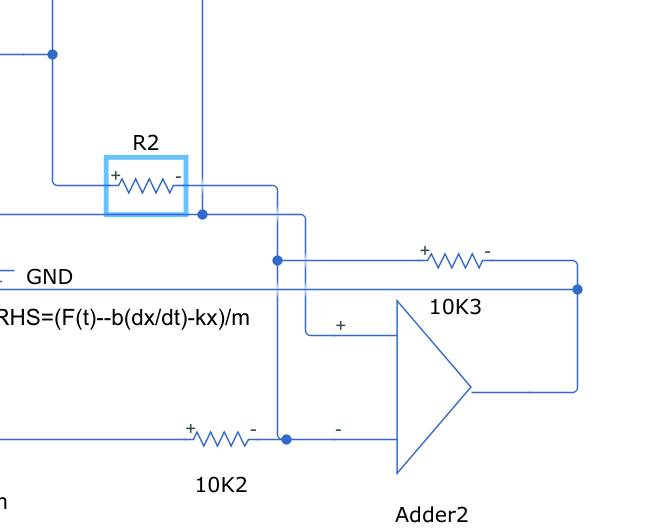
\includegraphics[width=0.5\textwidth]{pics/adder2-r2.png}
  \caption{Block diagram near \texttt{adder2}}
\end{figure}

I plotted $x(t)$ with different value of $R_2$ as belo in Figure \ref{pic-m-k}.

\begin{figure}
  \centering
  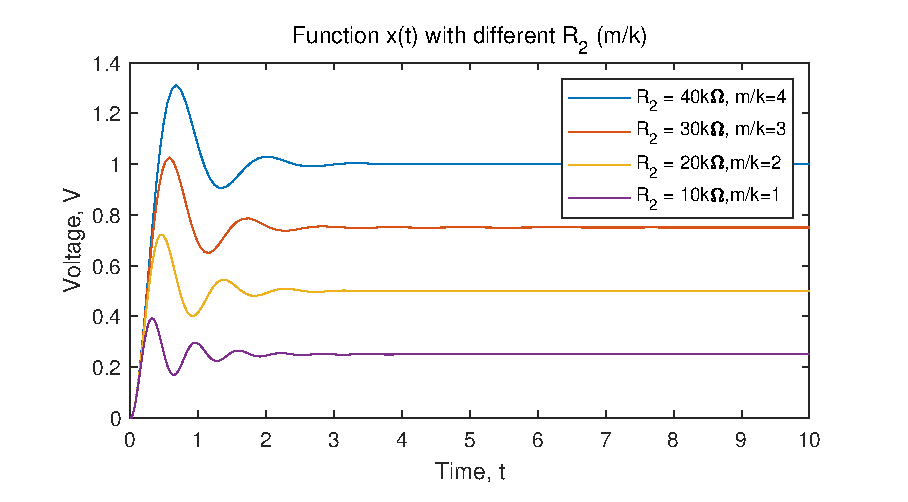
\includegraphics[width=0.7\textwidth]{pics/change-m-k.eps}
  \caption{Function $x(t)$ with different values of $\frac{m}{k}$}
  \label{pic-m-k}
\end{figure}

With increasing value of $R_2$, i.e. decreasing $k$,
\begin{enumerate}
  \item The system will reach its steady state with longer time.
  \item The frequency will decrease.
  \item The steady state value will increase, as $k$ changes the conditions
  at equilibrium.
\end{enumerate}

% End of Exercise 1
\pagebreak
\EXERCISENAME{2}{System Identification Experiment}
\subsubsection*{Hardware \& Software Setup}
After setting up both hardware and software I ran the simulation and obtained
the two plots (shown as Figure \ref{pic-ex2-step1} and \ref{pic-ex2-step2}),
following the instructions on lab manual.
\begin{figure}[h!]
  \begin{minipage}{0.49\linewidth} 
    \centering
    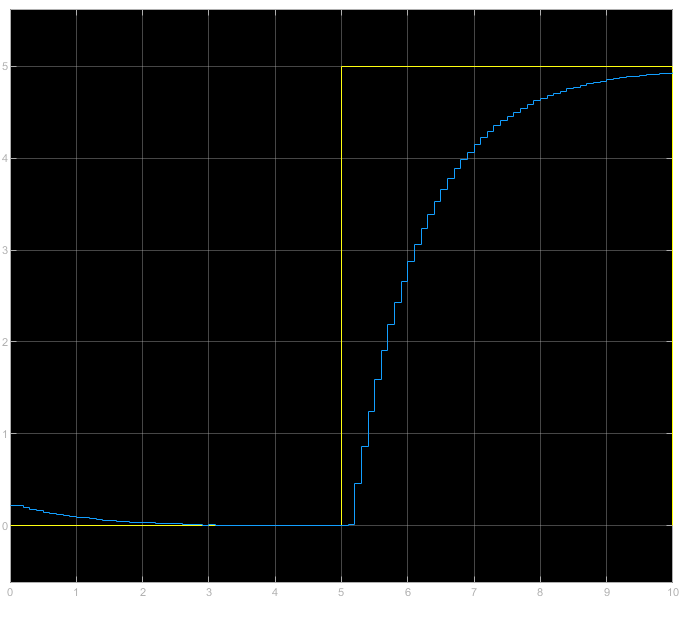
\includegraphics[width=\linewidth]{pics/arduino-voltage.png}
    \caption{Voltage output of Arduino}
    \label{pic-ex2-step1}
  \end{minipage}
  \begin{minipage}{0.49\linewidth}
    \centering
    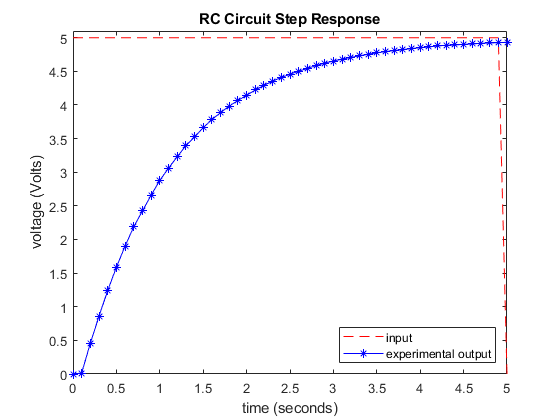
\includegraphics[width=0.9\linewidth]{pics/arduino-plotfigure.png}
    \caption{Voltage change within 5 seconds, generated by MATLAB}
    \label{pic-ex2-step2}
  \end{minipage}
\end{figure}

\subsubsection*{Parameter Identification}
To get the value of $\tau$, we have to find the time when the response reaches\
63.2\% of its total changes, i.e. \~3.16V.

From data gathered we find the response at 1.1s is 3.07V, and at 1.2s is 3.19V.
Using linear approximation we have 
\[V(t) = V(1.1) + \frac{V(1.2)-V(1.1)}{1.2-1.1}t = 3.07+1.2(t-1.1),
                                                          1.1\leq t \leq 1.2\]

Solving $V(t)=3.16$ we have $t\approx 1.175$s.
\end{document}
